\subsection{Anforderungsspezifikation}

\subsubsection{Funktionale Anforderungen}
In den folgenden Kapiteln werden jegliche funktionalen Anforderungen an die Applikation als sogenannte Use-Cases beschrieben. Als Übersicht dient das Use-Case-Diagramm, wie in Abbildung \ref{fig:ucmethode-635} dargestellt.

\paragraph{Brief Use-Cases}


\begin{figure}[h]
	\centering
	\makebox[\textwidth][c]{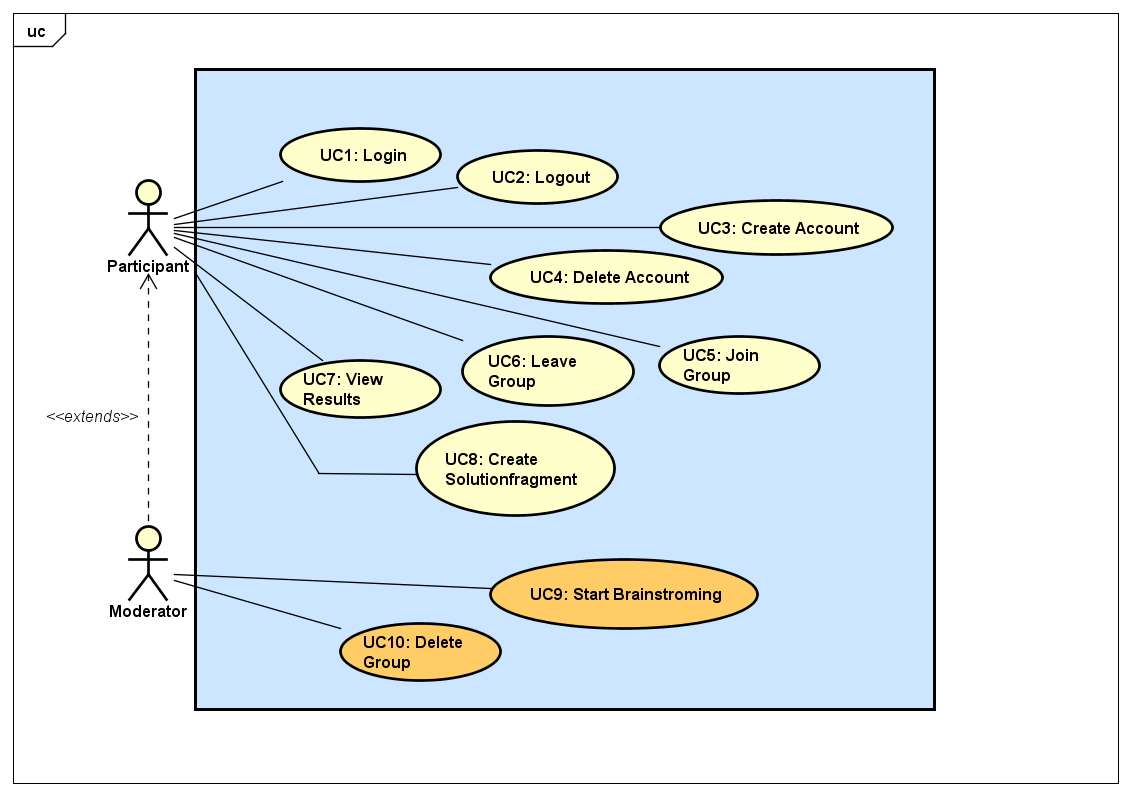
\includegraphics[width=1.2\linewidth]{img/anforderungen/UC-Methode635}}
	\caption{Use-Case-Diagramm}
	\label{fig:ucmethode-635}
\end{figure}

Jeder Use-Case hat den nachfolgend kurz (\textit{briefly}) beschriebenen  Funktionsumfang. Die Hauptaktivitäten UC7-9 sind am Schluss \textit{fully-dressed} beschrieben.

\begin{basedescript}{
		\desclabelstyle{\multilinelabel}
		\desclabelwidth{4.5cm}
		\setlength{\itemsep}{5ex}}
	\item[\textit{UC1: }Login] Als Participant möchte ich mich mit Benutzernamen und Passwort in das System einloggen können.
	
	\item[\textit{UC2: }Logout] Als eingeloggter Participant will ich mich ausloggen, sodass das Startfenster wieder erscheint.
	
	\item[\textit{UC3: }Create Account] Als Participant möchte ich mich registrieren können.
	
	\item[\textit{UC4: }Delete Account] Als Participant will ich meinen erstellten Account wieder löschen können.
	
	\item[\textit{UC5: }Join Brainstorming Team] Als Participant will ich einem bereits existierenden Team beitreten können.
	
	\item[\textit{UC6: }Leave Brainstorming Team] Als Participant will ich ein beigetretenes Team verlassen können.
	
	\item[\textit{UC7: }View Brainstorming Finding] Als Participant will ich, nachdem eine Brainstorming Session durchgeführt wurde, das Resultat (\textit{Finding}) meiner Gruppe einsehen können.
	
	\item[\textit{UC8: }Create Brainwave] Als Participant will ich während einer Brainstorming Session ein Brainwave (bestehend aus mehreren Ideen) erstellen und einreichen können. 
	
	\item[\textit{UC8a: }Insert Weblink] Als Participant will ich einen Weblink in mein aktuelles Sheet einfügen können.
	
	\item[\textit{UC8b: }Insert Picture] Als Participant will ich ein Bild in mein aktuelles Sheet einfügen können.
	
	\item[\textit{UC8c: }Insert Sketch] Als Participant will ich in mein aktuelles Sheet zeichnen können.
	
	\item[\textit{UC8d: }Insert Note] Als Participant will ich normalen Text in mein aktuelles Sheet einfügen können (Defaultoption).
	
	\item[\textit{UC9: }Start \\Brainstorming] Als Moderator will ich eine Brainstorming Session starten.
	
	\item[\textit{UC10: }Create Brainstorming Team] Als Moderator will ich 
	ein Brainstorming Team erstellen können. 
	
	\item[\textit{UC11: }Delete Brainstorming Team] Als Moderator will ich ein Brainstorming Team löschen können.
\end{basedescript}
\vspace{1cm}

\paragraph{Fully-Dressed Use-Cases}
Die fully-dressed Use-Cases folgen den im Modul \textit{Software Engineering 1} empfohlenen Punkten.
\renewcommand{\arraystretch}{1.35}
\begin{center}
	\begin{longtable}{| c | p{7cm} |}
		\hline
		\multicolumn{2}{|c|}{\textbf{Use Case 7: View Brainstorming Finding}}\\
		\hline\hline
		\textit{Primary Actor} & Participant\\
		\hline
		\textit{Stakeholders \& Interests} & Ein Participant wünscht sich eine Übersicht von allen Ideen der Gruppenmitglieder. Er will das Gesamtresultat (\textit{Brainstorming Finding}) einsehen und daraus etwas lernen. \\
		\hline
		\textit{Preconditions} & Participant existiert im System (UC3), ist eingeloggt (UC1) und einer Gruppe beigetreten (UC5). Zudem hat die Gruppe des Participants alle Runden durchgemacht.\\
		\hline
		\textit{Post Conditions/Success Guarantee} & Die Notizen aller Participants werden übersichtlich dargestellt. Das heisst, jede Ausgangsidee ist mit deren Ergänzungen von den verschiedenen Participants ersichtlich.\\
		\hline
		\textit{Main Success Scenario/Basic Flow} & 
		\begin{enumerate}[noitemsep]
			\item Der Participant schliesst die abschliessende Runde als Letzter ab.
			\item Das System speichert seine Notizen auf dem Server.
			\item Das System zeigt dem Participant eine Meldung, dass das Finding einsehbar ist.
			\item Der Participant clickt auf "Resultate einsehen" (o.Ä.).
			\item Das System zeigt dem Participant eine Übersicht mit allen Notizen der Teilnehmer.
		\end{enumerate}\\
		\hline
		\textit{Alternative Flows} &
		Alternative	Success Scenario 1:
		\begin{enumerate}[label=1.\alph*,noitemsep]
			\item Der Participant schliesst die Runde nicht als Letzter ab.
			\item Das System speichert seine Notizen auf dem Server und zeigt dem Benutzer die verbleibende Zeit an.
			\item Der Participant aktualisiert den gezeigten Screen nach dem Ablauf der Zeit.
		\end{enumerate}
		Alternative Success Scenario 2:
		\begin{enumerate}[label=4.\alph*,noitemsep]
			\item Der Participant clickt nicht auf "Resultate einsehen", sondern navigiert zurück auf den Homescreen.
			\item Das System zeigt dem Participant den Homescreen an.
			\item Der Participant navigiert auf seine Gruppe.
			\item Das System zeigt dem User die Gruppe an.
			\item Der Participant will sich die Resulate dieser Gruppe anzeigen lassen und clickt entsprechenden Button.
			\item Das System zeigt dem Benutzer die Übersicht an.
		\end{enumerate}\\
		\hline
		\textit{Frequency of Occurrence} & Oft, Kernfunktionalität\\
		\hline
	\end{longtable}
\end{center}



\renewcommand{\arraystretch}{1.35}
\begin{center}
	\begin{longtable}{| c | p{7cm} |}
		\hline
		\multicolumn{2}{|c|}{\textbf{Use Case 8: Create Brainwave}}\\
		\hline\hline
		\textit{Primary Actor} & Participant\\
		\hline
		\textit{Stakeholders \& Interests} & Ein Participant will, dass seine Brainwave erfasst wird. \\
		\hline
		\textit{Preconditions} & Der Participant muss existent (UC3) sowie eingeloggt (UC1) sein. Des Weiteren muss ein Brainstorming Team existieren (UC10), zu welchem er gehört. Die Brainstorming Runde muss ebenfalls gestartet worden sein (UC9). \\
		\hline
		\textit{Post Conditions/Success Guarantee} & Vom Participant erfasste Notizen werden erfolgreich auf dem System gespeichert. \\
		\hline
		\textit{Main Success Scenario/Basic Flow} & 
		\begin{enumerate}[noitemsep]
			\item Der Participant erfasst während der aktuellen Rundenzeit Notizen.
			\item Das System zeigt diese Notizen an.
			\item Der Participant beendet frühzeitig die Runde und clickt auf "Brainwave abgeben" (o.Ä).
			\item Das System persistiert die Notizen und zeigt dem Participant eine Bestätigung an. 
			\item Der Benutzer kann aktualisieren, um den nächsten Rundenstart nicht zu verpassen.
		\end{enumerate}\\
		\hline
		\textit{Alternative Flows} &
		Alternative	Success Scenario 1:
		\begin{enumerate}[label=3.\alph*,noitemsep]
			\item Der Participant beendet die Runde nicht manuell.
			\item Das System zeigt dem Participant eine Meldung an, dass die Zeit der Runde abgelaufen ist. Es persistiert die bis zu dem Zeitpunkt erfassten Notizen.
		\end{enumerate}\\
	
		\hline
		
		\textit{Frequency of Occurrence} & Sehr oft, passiert pro Brainstorming-Session mehrmals.\\
		
		\hline
	\end{longtable}
\end{center}


\renewcommand{\arraystretch}{1.35}
\begin{center}
	\begin{longtable}{| c | p{7cm} |}
		\hline
		\multicolumn{2}{|c|}{\textbf{Use Case 9: Start Brainstorming}}\\
		\hline\hline
		\textit{Primary Actor} & Moderator\\
		\hline
		\textit{Stakeholders \& Interests} & Ein Moderator will eine neue Brainstorming-Session starten können. \\
		\hline
		\textit{Preconditions} & Der Moderator muss existent (UC3) sowie eingeloggt (UC1) sein. Des Weiteren muss ein Brainstorming Team existieren (UC10), das er erstellt hat. Zudem muss die Gruppe komplett sein (konfigurierte Anzahl an Participants sind dem Team beigetreten). \\
		\hline
		\textit{Post Conditions/Success Guarantee} & Alle Participants des Teams können aktualisieren und sehen die gestartete Runde. \\
		\hline
		\textit{Main Success Scenario/Basic Flow} & 
		\begin{enumerate}[noitemsep]
			\item Der Moderator clickt auf "Brainstorming starten" (o.Ä) auf der Gruppe, die er erstellt hat. 
			\item Das System überprüft, dass alle Einstellungen korrekt sind und die korrekte Anzahl an Participants in der Gruppe sind. 
			\item Das System zeigt dem Moderator an, dass die Session gestartet ist.
			\item Der Moderator kann wie die normalen Participants eine Brainwave (bestehend aus mehreren Ideen) erfassen.
		\end{enumerate}\\
		\hline
		\textit{Alternative Flows} & -\\
		
		\hline
		
		\textit{Frequency of Occurrence} & Oft, Kernfunktionalität.\\
		
		\hline
	\end{longtable}
\end{center}




\paragraph{Abuse-Cases}
%Abuse cases?
Um einem Missbrauch der Applikation entgegenzuwirken, sind neben den Use-Cases auch Abuse-Cases definiert. Diese helfen, mit unangebrachtem Inhalt und unangebrachter Verwendung umzugehen.
\begin{basedescript}{%
		\desclabelstyle{\multilinelabel}
		\desclabelwidth{4.5cm}}
	\item[\textit{AC1: }Unangebrachte Brainwaves] Ein Participant könnte unangebrachte \footnote{Als unangebrachte Inhalte werden Brainwaves mit rassistischen, pornographischen, sexistischen sowie unethischen Inhalten verstanden.} Inhalte in einer Gruppe hinzufügen. Um dies zu verhindern, könnte eine die Applikation um eine Funktion erweitert werden, die es dem Moderator erlaubt, Benutzer auszuschliessen.
	
	\item[\textit{AC2: }Missbrauch der Vertraulichkeit] Ein Participant könnte das Brainstorming Finding an die Konkurrenz leaken. 
\end{basedescript}

%Sequence diagram
\paragraph{Sequenzdiagramm}
Der Ablauf der Kernlogik ist der Abbildung \ref{fig:seq-methode635} zu entnehmen. Darin ist der Prozess vom Erstellen des BrainstormingTeams (UC10) bis zum Abschliessen der Brainwave modelliert.
\begin{figure}[h]
	\centering
	\makebox[\textwidth][c]{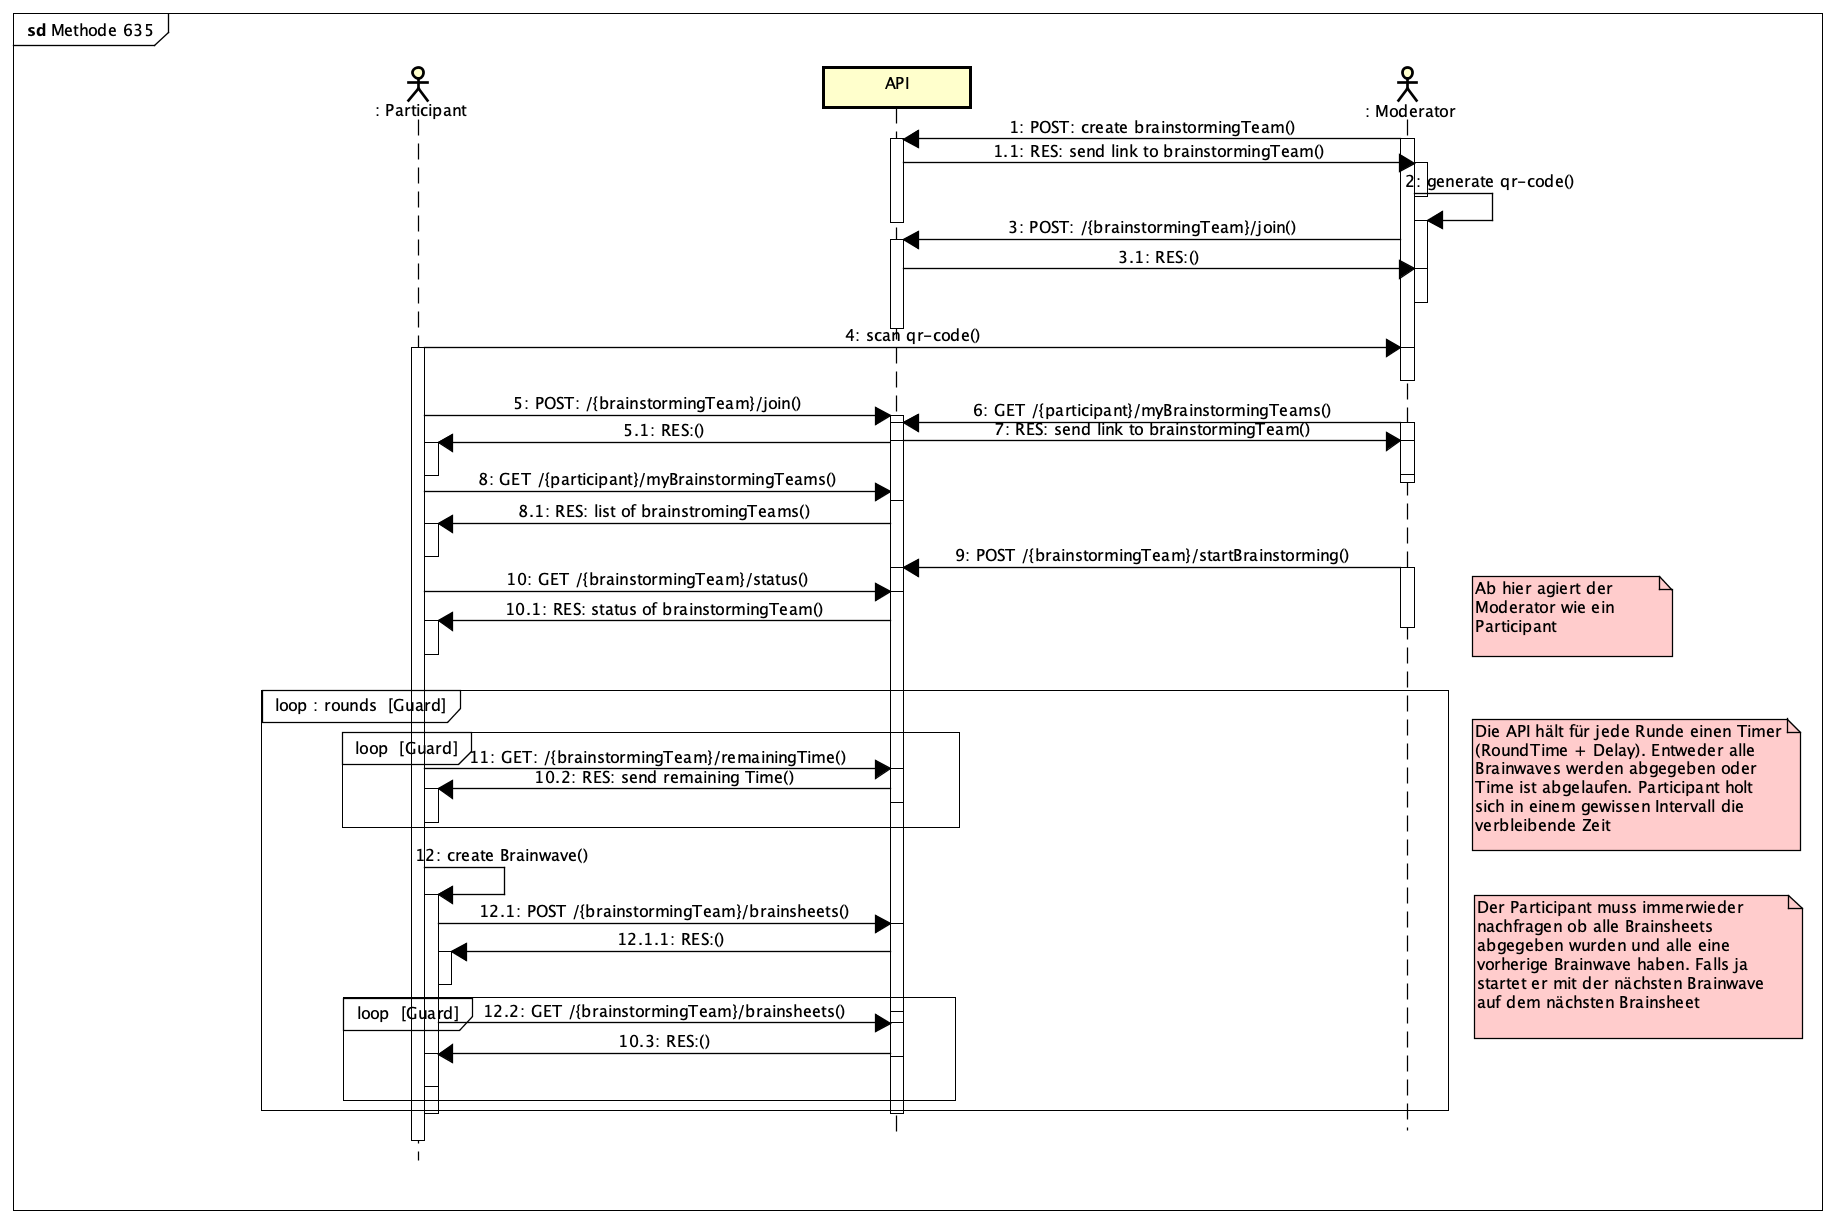
\includegraphics[width=1\linewidth]{img/anforderungen/Seq-Methode635}}
	\caption{Ablauf der Kernlogik}
	\label{fig:seq-methode635}
\end{figure}


\subsubsection{Nicht-Funktionale Anforderungen}
Beim Thema Nicht-Funktionale Anforderungen halten wir uns an die Standards ISO 9126\cite{ISO9126} bzw. dessen Nachfolger ISO 25010\cite{ISO9126_ISO25010}. Beide ISO-Normen sind sich sehr ähnlich und liefern eine gute Checkliste für jegliche Art von Systemanforderungen.

\begin{figure}[h]
	\centering
	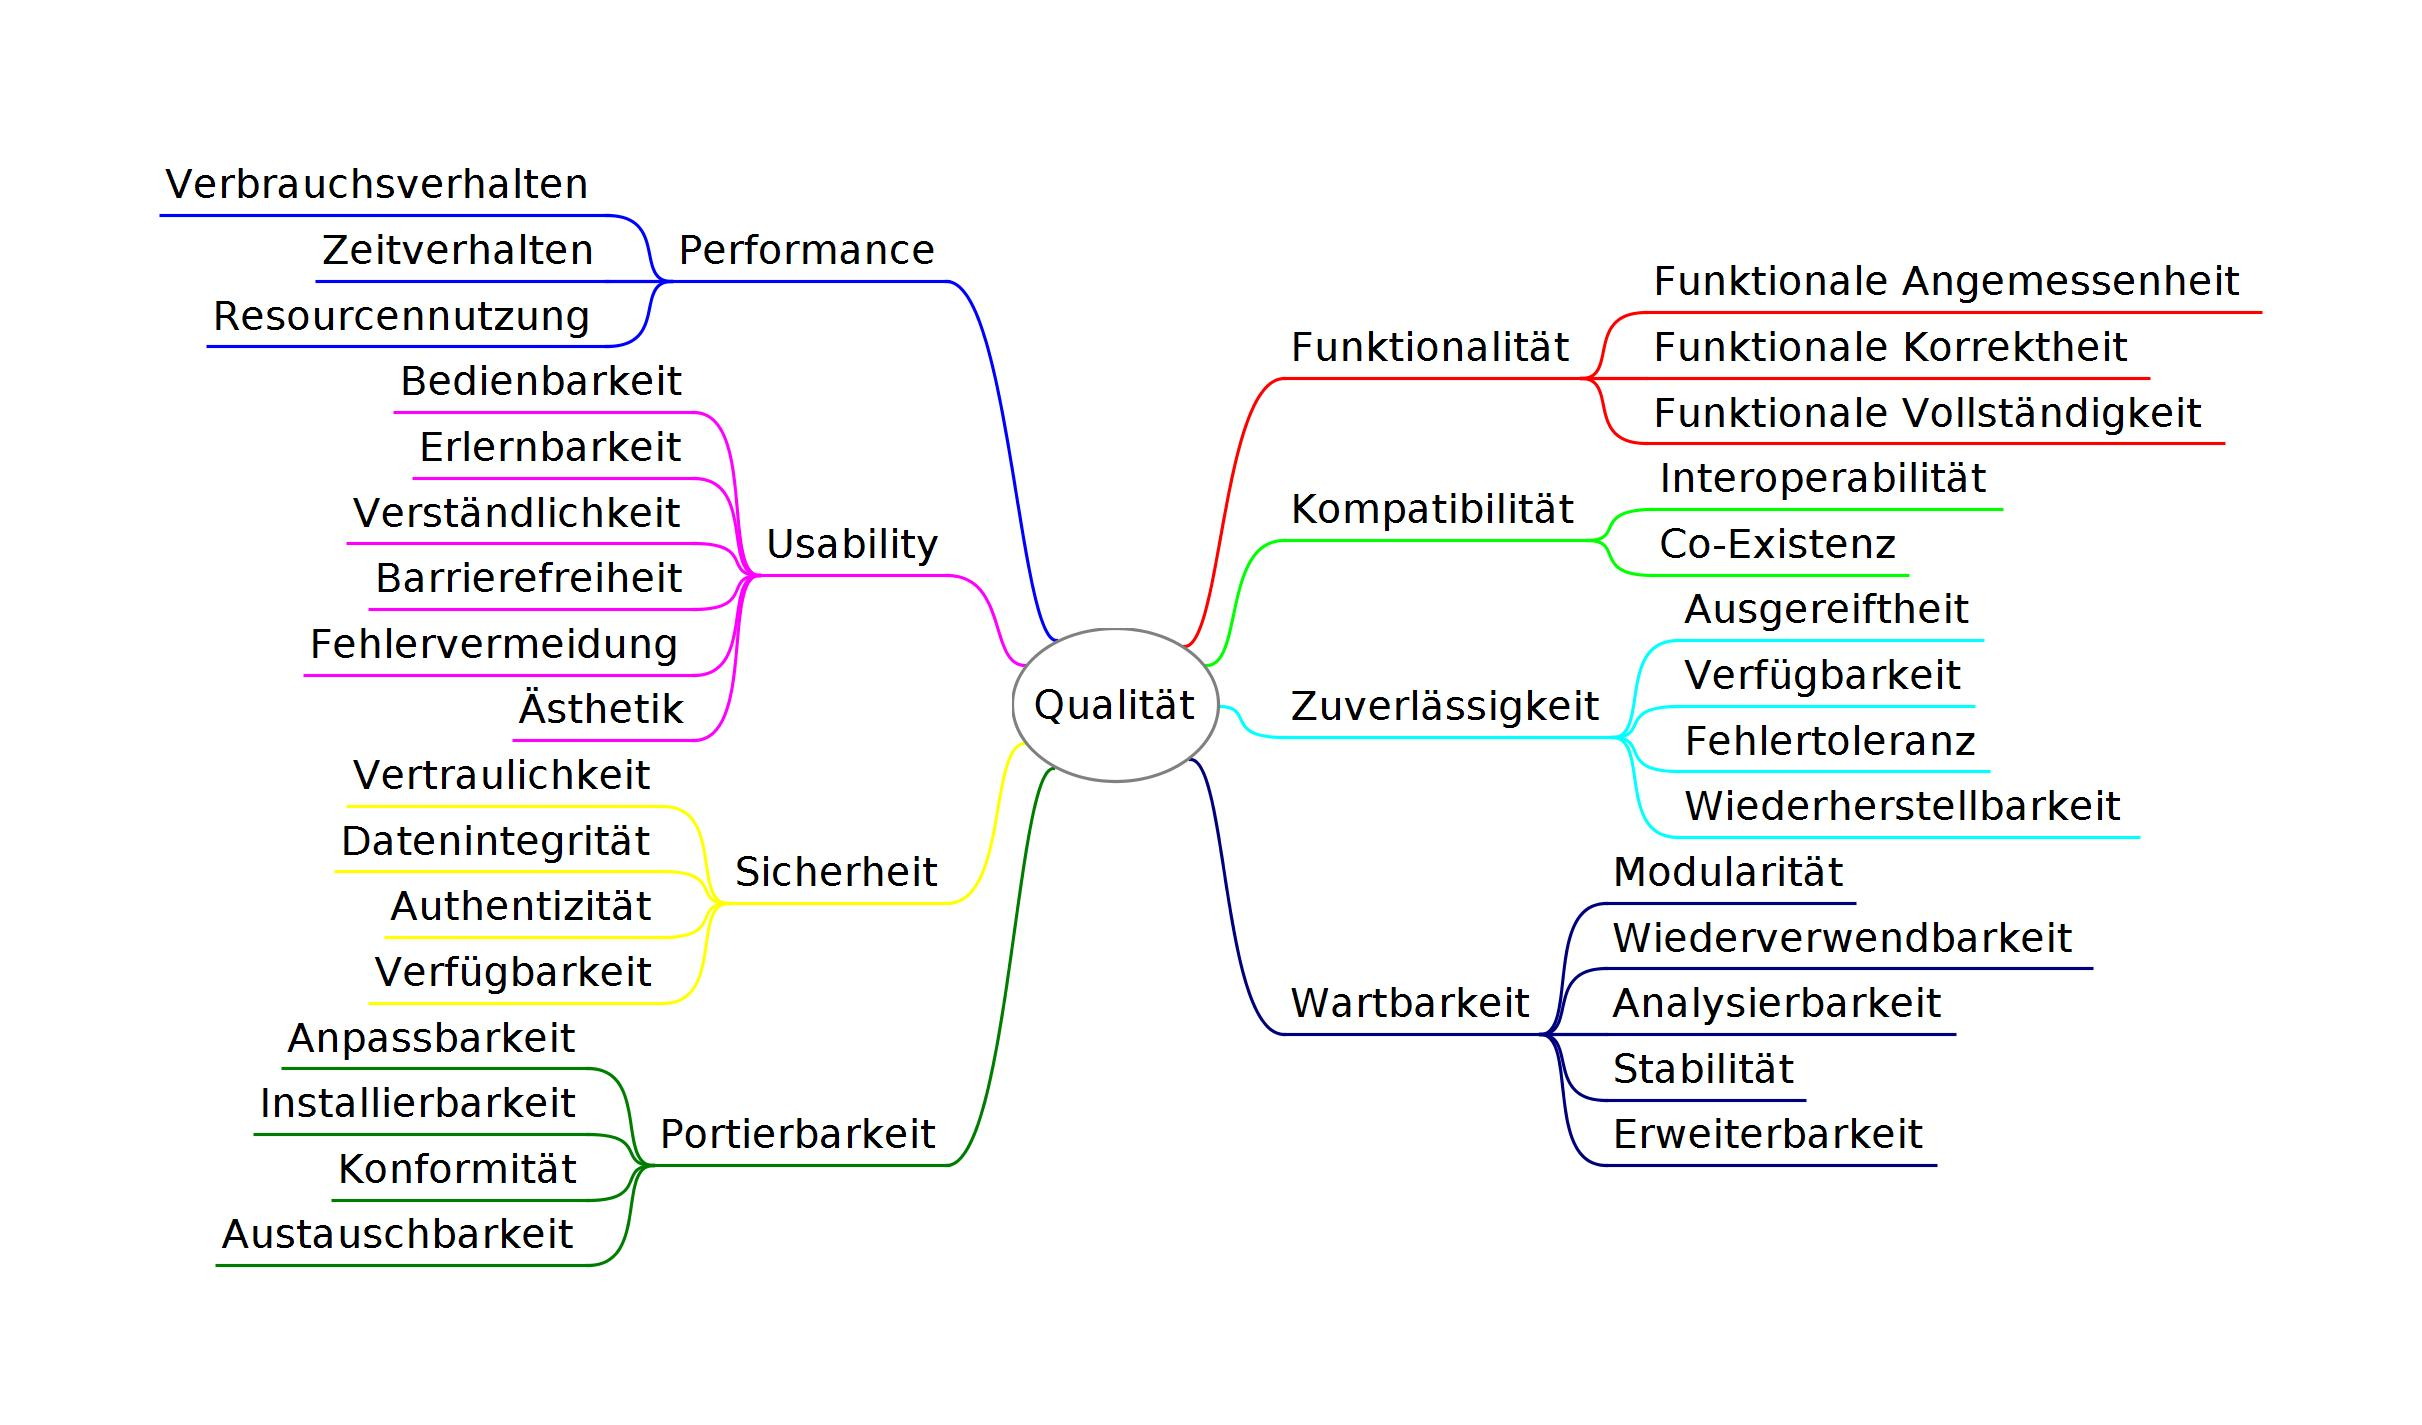
\includegraphics[width=1\linewidth]{img/anforderungen/quality}
	\caption[Anforderungskategorien nach ISO 25010]{Anforderungskategorien nach  ISO 25010}\cite{ISO25010_Bild}
	\label{fig:ISO 25010}
\end{figure}

Diese Normen sind sehr umfangreich gestaltet. Wir werden uns daher auf die, für uns, wichtigsten Anforderungen konzentrieren. Um genaue und erfüllbare nicht-funktionale Anforderungen zu definieren, müssen die SMART-Kriterien \cite{SMART} erfüllt sein. 

\begin{description}[leftmargin=!,labelwidth=\widthof{\bfseries Wiederverwendbarkeit}]
	\item[Ressourcennutzung] Die internen Ressourcen Kamera, Dateisystem dürfen nur bei effektivem Bedarf benützt werden. Die CPU-Ressourcen\-nutzung darf pro Minute im Bereich von bis zu 40\% in Anspruch genommen werden.\footnote{Referenzsystem Android: Huawei P10 mit Android Version 8.0.0 mit Hisilicon Kirin 960 CPU und 4GB RAM}\footnote{Referenzsystem iOS: iPhone 6 mit iOS Version 12 mit Dual-core 1.4 GHz Typhoon CPU und 1GB RAM}
	
	\item[Bedienbarkeit] Wenn eine Aktion länger als 1-2s geht, soll dem User ein Wartesymbol angezeigt werden. 
	
	\item[Ästhetik] Die Benutzeroberflächen der Applikation sind so gestaltet, dass die Elemente wiedererkennbar sind (Buttons haben gleichen Stil, leere Textfelder haben Platzhalter). 
	
	\item[Vertraulichkeit] Die Daten einer Brainstorming Session können nur von der zugehörigen Gruppe eingesehen werden. 
	
	\item[Anpassbarkeit] Die Anpassung bestehender oder Integration neuer Brain\-storming-Methoden muss gewährleistet sein.
	
	\item[Installierbarkeit] Die Installation der Applikation auf einem Endgerät erfolgt durch das Ausführen eines *.apk oder *.ipa.\footnote{Eine Applikation auf einem Android Smartphone hat üblicherweise die Endung *.apk. Beim iPhone bzw. beim iOS haben die einzelnen Applikationen die Endung *.ipa.} Dieser Prozess soll unter 1 Minute geschehen.
	
	\item[Co-Existenz] Sollte zu einem späteren Zeitpunkt entschieden werden ein Web-Frontend zu programmieren, muss dieses co-existent mit der Xamarin Applikation existieren können.
	
	\item[Wiederherstellbarkeit] Im Falle eines fehlerhaften Features, muss es innerhalb eines Werktages möglich sein, die Applikation wieder auf den letzten funktionierenden Stand zurück zu holen und erneut zu deployen.	
	
	\item[Wiederverwendbarkeit] Die Auswertung von 'Duplicated Code' in SonarQube soll im Bereich zwischen 5-10\% \cite{Duplicated_Code} liegen. Dies deutet auf eine hohe Wiederverwendbarkeit hin, denn ansonsten müsste der Code kopiert werden. 
	
	%TODO: Referenz auf Use Cases
	\item[Analysierbarkeit] Das Ausführen eines Use-Cases muss durch Analyse von Logfiles erkennbar sein.
\end{description}
